\chapter{DESIGN AND ANALYSIS}\label{chap-design}
\thispagestyle{empty}

The design phase incorporated detailed selection, calculation, and validation of the high voltage components required to achieve efficient and stable plasma generation. The main objective of the design is to deliver a controlled high-frequency high-voltage signal to the plasma electrodes while ensuring safety, efficiency, and adaptability for different applications. In this chapter, we discuss the system block diagram and the design steps of UCC driver, transformer, and voltage multiplier. The UCC gate driver IC, transformer, and voltage multiplier form a critical part of the isolation and fast-switching capability of the system. An improper design in this stage can lead to delayed switching, power losses, or damage to the MOSFETs. 

\section{System Block Diagram}

The block diagram provides a high-level overview of the electrical architecture used in the cold plasma generator. The system is powered by a 230~V~AC mains supply, which is regulated and converted into different DC voltage levels required for the operation of various components.  

\begin{figure}[H]
\centering
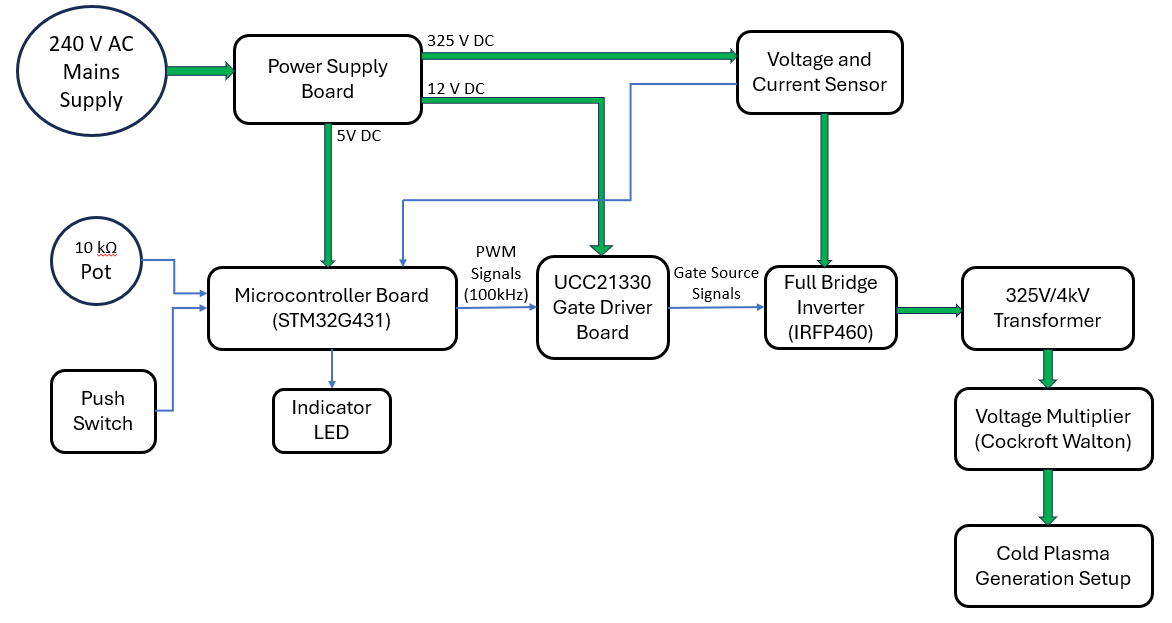
\includegraphics[width=1\linewidth]{./picture-files/blockdia.png}
\caption[Block Diagram of System]{Block Diagram of System}
\label{fig-block}
\end{figure}


\begin{itemize} 
 \item \textbf{Power Supply Modules:}  
The 230~V~AC input is stepped down and rectified into three key DC voltage levels:
\begin{itemize} 
 \item 5~V~DC: Used to power the microcontroller.
 \item 12--15~V~DC: Used for the gate driver circuit.
 \item 320~V~DC: Used as the primary input for the power converter and high-voltage generation.
\end{itemize}

\begin{figure}[h!]
\centering
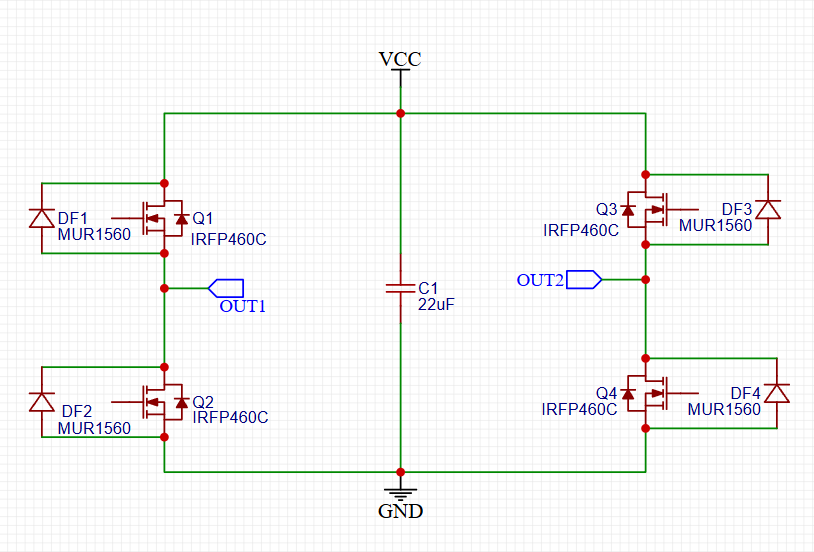
\includegraphics[width=1\linewidth]{./picture-files/hbridge-schematic1.png}
\caption[Schematic of IRFP460 H-Bridge]{H-Bridge schematic used to drive high-voltage transformer}
\label{fig-hbridge}
\end{figure}

 \item \textbf{Microcontroller:}  
STM32G431-Long Core Demo Board is used for controlling the system's switching logic. It generates PWM signals at 100 kHz to drive the high voltage circuit with precise control over frequency and duty cycle, enabling modulation of the plasma output. It also takes feedback from the system.

 \item \textbf{Gate Driver Circuit:}  
This circuit acts as an interface between the microcontroller and the power stage. It amplifies the logic-level signals from the microcontroller to levels suitable for driving the power MOSFETs or IGBTs used in the H-Bridge converter.

\item \textbf{Voltage and Current Sensor:}
This module senses the input voltage and current from the DC bus and send it to the microcontroller.



 \item \textbf{H Bridge Circuit:}  
The power converter, typically an H-Bridge topology implemented using IRFP460 MOSFETS, is responsible for converting the DC voltage into high-frequency AC. This AC signal is necessary for driving the high-voltage transformer.

 \item \textbf{High-Voltage Transformer:}  
The transformer steps up the AC voltage from tens of volts to several kilovolts (kV) needed for plasma generation.

 \item \textbf{Voltage Multiplier:}  
A voltage multiplier circuit (e.g., Cockcroft--Walton) further increases the AC voltage output of the transformer to reach the target level of approximately 30~kV~DC, required to initiate and sustain the cold plasma discharge.
\end{itemize}

\section{System Design}

In this project, five main subsystems were designed:  
\begin{enumerate}
    \item \textbf{UCC21330 isolated gate driver circuit} for driving IRFP460 MOSFETs in the H-bridge.  
    \item \textbf{Power Supply Board} for supplying power to the inverter, gate driver and the microcontroller.
    \item \textbf{Non discharge RCD snubber} for protecting inverter MOSFETs against overvoltage.
    \item \textbf{High voltage step-up transformer}, which interfaces the H-bridge to the Cockcroft--Walton voltage multiplier.  
    \item \textbf{Cockcroft--Walton multiplier}, which provides the final 30~kV~DC required for plasma excitation. 
\end{enumerate}

\subsection{UCC21330 Gate Driver Design}
\label{sec:ucc21330}

This section documents the design calculations and chosen components for the UCC21330 isolated gate driver used to drive the IRFP460 MOSFETs in the H-bridge.


\begin{figure}[h!]
\centering
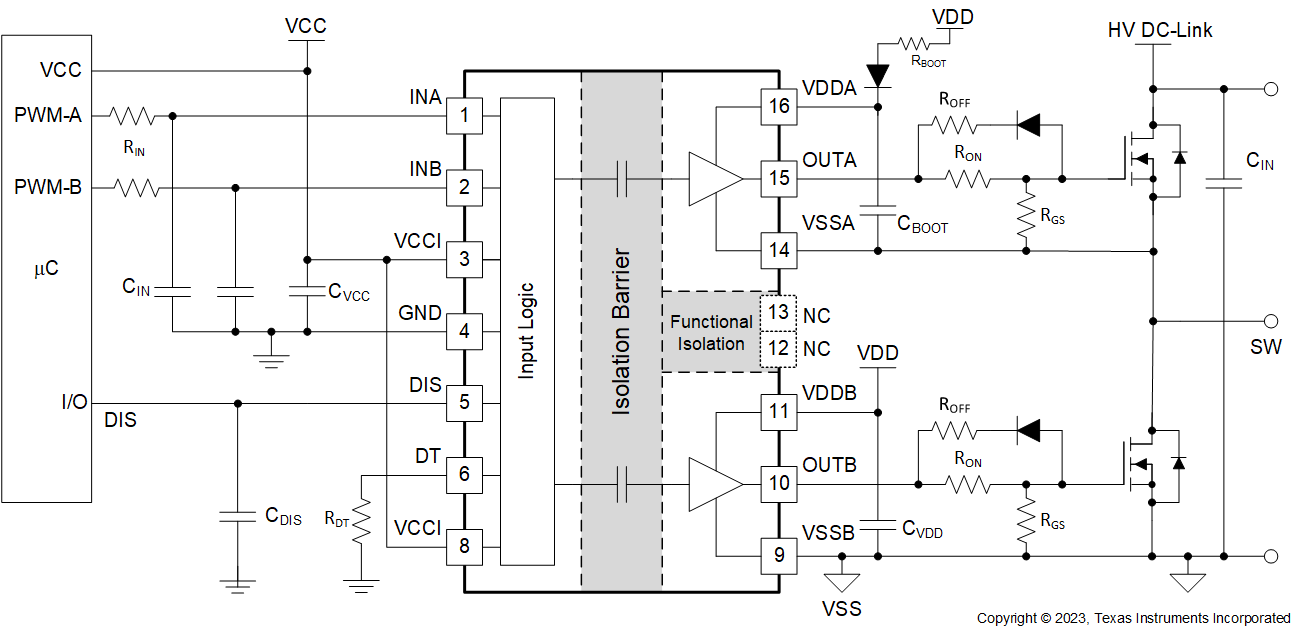
\includegraphics[width=1\linewidth]{./picture-files/ucc.png}
\caption[Schematic of UCC21330 Driver]{Application Schematic of UCC21330 Driver for H-Bridge}
\caption*{Source: Texas Instruments, UCC21330 Datasheet}
\label{fig-ucc}
\end{figure}


\subsubsection{Input RC (Noise / Input Filtering)}
\[
R_{\mathrm{in}} = \SI{51}{\ohm}, \qquad C_{\mathrm{in}} = \SI{33}{\pico\farad}
\]

\[
f_{\mathrm{cutoff}} = \frac{1}{2\pi R_{\mathrm{in}} C_{\mathrm{in}}} \approx \SI{94.6}{\mega\hertz}
\]

\subsubsection{Dead-time resistor ($R_\text{Dt}$)}
\[
t_{dt} = 8.6\,R_\text{Dt} + 13~\text{ns}, \quad t_{dt} = \SI{200}{ns}
\]

\[
R_\text{Dt} = \frac{t_{dt} - 13}{8.6} \approx \SI{22}{\kilo\ohm}
\]

\subsubsection{Bootstrap diode and series resistor ($R_\text{BOOT}$)}
\[
I_\text{Dboot} = \frac{V_{DD} - V_\text{BDf}}{R_\text{BOOT}}, \quad V_\text{DD} = \SI{15}{V}, \; V_\text{BDf} \approx \SI{1.05}{V}
\]

\[
R_\text{BOOT} \approx \SI{18}{\ohm} \text{ (2 W)}
\]

Recommended bootstrap diode: MUR460.

\subsubsection{Bootstrap capacitor ($C_\text{BOOT}$)}
\[
Q_\text{total} = Q_g + \frac{I_{VDD}}{f_{sw}} \approx \SI{235}{nC}, \quad \Delta V_\text{DDA} = \SI{0.5}{V}
\]

\[
C_\text{BOOT} = \frac{Q_\text{total}}{\Delta V_\text{DDA}} \approx \SI{470}{nF}
\]

Practical implementation: \SI{470}{\nano\farad} MLCC in parallel with \SI{1}{\micro\farad}.


\subsubsection{Estimated Gate-Driver Switching Loss}
\[
P_{G\_SW} = 2 \cdot V_{pp} \cdot Q_g \cdot f_{sw} \approx \SI{0.63}{W}
\]

\subsubsection{Design summary table}
\begin{table}[h!]
\centering
\caption{Selected components and values for UCC21330 gate driver}
\label{tab:ucc-components}
\begin{tabular}{@{} l l l  @{}}
\toprule
Parameter / Part & Value & Notes \\
\midrule
$R_{\mathrm{in}}$ & \SI{51}{\ensuremath{\Omega}} & Input series resistor, 0805/1206 \\
$C_{\mathrm{in}}$ & \SI{33}{\pico\farad} & Input filter capacitor \\
$R_{\mathrm{Dt}}$ & \SI{22}{\kilo\ensuremath{\Omega}} & Dead-time set resistor \\
$R_{\mathrm{BOOT}}$ & \SI{18}{\ensuremath{\Omega}}, \SI{2}{\watt} & Bootstrap series resistor \\
$C_{\mathrm{BOOT}}$ & \SI{470}{\nano\farad} + \SI{1}{\micro\farad} & MLCC, \SI{50}{\volt} \\
Bootstrap diode & MUR460 & \SI{600}{\volt}, fast \\
Turn-off diode & UF4007 & Fast rectifier \\
Gate resistor & \SI{10}{\ensuremath{\Omega}} & Ron/Roff applied at gate \\
Discharge resistor & \SI{10}{\kilo\ensuremath{\Omega}} & Pull-down on gate \\
$P_{G\_SW}$ & \SI{0.63}{\watt} & Dynamic switching dissipation \\
\bottomrule
\end{tabular}
\end{table}




\subsubsection{Practical PCB notes}
\begin{itemize}
  \item Place the bootstrap capacitor and decoupling capacitors close to UCC21330 pins.
  \item Keep gate loop inductance low.
  \item Ensure proper creepage/clearance for high-voltage areas.
\end{itemize}



\subsection{Power Supply Board Design}
\label{subsec:powerdesign}

The designed power supply board provides three independent DC voltage rails required for the operation of the inverter bridge system:

\begin{itemize}
\item \textbf{5 V DC} – Used for supplying the STM32 microcontroller and the low voltage logic side of the UCC21330 gate driver.
\item \textbf{12 V DC} – Used to power the high side and low side gate driver circuits of the UCC21330 for driving the MOSFET bridge.
\item \textbf{320 V DC} – Used as the high voltage DC link supply for the full bridge power stage.
\end{itemize}

The 5 V and 12 V supplies are generated using isolated AC-DC modules:

\begin{itemize}
\item Hi-Link HLK-10M05 (5 V, 10 W)
\item Hi-Link HLK-10M12 (12 V, 10 W)
\end{itemize}

Since these modules provide regulated isolated outputs, no additional complex design was required for these sections. Therefore, the major design effort focuses on the \textbf{320 V DC mains rectifier stage}, which supplies the high power DC link of the inverter.

The rectifier stage is designed to support a maximum power of:

\[
P_{max} = 300\,W
\]

For a DC link voltage of approximately:

\[
V_{DC} \approx 320V
\]

The maximum DC current drawn from the rectifier becomes:

\[
I_{DC} = \frac{P}{V} = \frac{300}{320} \approx 0.94\,A
\]

Thus the rectifier stage was designed for approximately \textbf{1 A continuous DC current}.

\subsubsection{Bridge Rectifier Selection}

The AC mains is rectified using the \textbf{GBJ2506 bridge rectifier}.  
This rectifier was selected due to the following reasons:

\begin{itemize}
\item Maximum repetitive reverse voltage: \textbf{600 V}
\item Average rectified output current: \textbf{25 A}
\item High surge current capability
\item Integrated bridge configuration simplifying PCB layout
\end{itemize}

Although the expected continuous load current is only about \textbf{1 A}, a rectifier with significantly higher current rating was selected to handle:

\begin{itemize}
\item Capacitor charging surge currents
\item Possible transient overload conditions
\item Improved thermal reliability
\end{itemize}

The rectifier converts the 230 V AC mains into an approximate peak DC voltage:

\[
V_{DC} = \sqrt{2} \times V_{AC}
\]

\[
V_{DC} = 1.414 \times 230 \approx 325\,V
\]

Thus the DC link voltage of the system is approximately \textbf{320–325 V DC}.

\subsubsection{Input EMI Filter Choke}

To reduce conducted electromagnetic interference and suppress high frequency noise entering or leaving the converter, a line choke is used.

The selected component is:

\begin{center}
\textbf{Würth Elektronik 7448258022}
\end{center}

Specifications:

\begin{itemize}
\item Inductance: \textbf{2.2 µH}
\item Rated current: \textbf{8 A}
\end{itemize}

This choke helps in:

\begin{itemize}
\item Limiting high frequency switching noise
\item Reducing differential mode EMI
\item Improving overall power supply stability
\end{itemize}

\subsubsection{Input Line Filtering Capacitors}

Two capacitors are used at the input stage for noise suppression:

\begin{itemize}
\item \textbf{0.33 µF} line filtering capacitor
\item \textbf{0.1 µF / 280 V} capacitor across the AC line
\end{itemize}

These capacitors work together with the input choke to form an LC filter that attenuates high frequency noise components generated by the inverter stage.

\subsubsection{Inrush Current Limiting}

When the power supply is first connected to the mains, the large DC link capacitors appear as a short circuit. This results in a very high instantaneous current known as \textbf{inrush current}.

To limit this current, an NTC thermistor is used:

\begin{center}
\textbf{NTC 15D20}
\end{center}

Specifications:

\begin{itemize}
\item Cold resistance: \textbf{15 $\Omega$}
\item Diameter: \textbf{20 mm}
\end{itemize}

\paragraph{Inrush Current Calculation}

At startup the DC link capacitors are completely discharged.

Peak rectified voltage:

\[
V_{peak} = 325V
\]

Initial inrush current:

\[
I_{inrush} = \frac{V}{R}
\]

\[
I_{inrush} = \frac{325}{15}
\]

\[
I_{inrush} \approx 21.6A
\]

Thus the NTC limits the initial surge current to approximately \textbf{22 A}. As the thermistor heats up, its resistance drops significantly, allowing normal operating current to flow with minimal losses.

\subsubsection{Fuse Protection}

A \textbf{5 A, 230 V AC fuse} is used at the mains input for protection.

The fuse provides protection against:

\begin{itemize}
\item Short circuits
\item Component failure
\item Excessive current draw
\end{itemize}

The fuse rating is chosen such that it can withstand normal operating currents but will disconnect the circuit during abnormal conditions.

\subsubsection{DC Link Capacitor Design}

The rectified output is filtered using electrolytic capacitors.


\paragraph{Ripple Voltage Design}

The DC link ripple was limited to \textbf{3\%} of the output voltage.

\[
V_{ripple} = 0.03 \times 320
\]

\[
V_{ripple} = 9.6V
\]

For a full bridge rectifier the ripple capacitor equation is:

\[
C = \frac{I}{2f\Delta V}
\]

where

\begin{itemize}
\item $I$ = load current
\item $f$ = mains frequency (50 Hz)
\item $\Delta V$ = ripple voltage
\end{itemize}

\[
C = \frac{0.94}{2 \times 50 \times 9.6}
\]

\[
C \approx 979 \mu F
\]

Thus approximately \textbf{1000 µF} capacitance is required to maintain 3\% ripple.

Capacitors used on the power supply board:

\begin{itemize}
\item 2 × 470 µF, 450 V
\end{itemize}

Additionally, on the inverter bridge board:

\begin{itemize}
\item 1 × 470 µF, 450 V
\end{itemize}

Thus the total capacitance becomes:

\[
C_{total} = 470 + 470 + 470
\]

\[
C_{total} = 1410 \mu F \approx 1500 \mu F
\]

Since the implemented capacitance is approximately \textbf{1500 µF}, the ripple voltage becomes:

\[
\Delta V = \frac{I}{2fC}
\]

\[
\Delta V = \frac{0.94}{2 \times 50 \times 1500 \times 10^{-6}}
\]

\[
\Delta V \approx 6.27V
\]

Thus the actual ripple percentage is:

\[
\frac{6.27}{320} \times 100 \approx 1.96\%
\]

Therefore the implemented design provides a ripple significantly lower than the initial design requirement.

\subsubsection{Bleeder Resistor Design}

To safely discharge the DC link capacitors after the power supply is turned off, bleeder resistors are used.

The design uses:

\begin{itemize}
\item 2 × 47 k$\Omega$
\item Power rating: 2 W each
\end{itemize}

These resistors are connected in series across the DC link.

Equivalent resistance:

\[
R = 47k + 47k
\]

\[
R = 94k\Omega
\]

\subsubsection{RC Time Constant}

\[
\tau = RC
\]

\[
\tau = 94000 \times 0.0015
\]

\[
\tau \approx 141\,s
\]

The voltage decay follows:

\[
V(t) = V_0 e^{-t/\tau}
\]

A capacitor typically discharges to a safe level after approximately $5\tau$


\[
5\tau \approx 705s \approx 11.75\,minutes
\]

The discharge time is intentionally kept relatively long in order to:

\begin{itemize}
\item Minimize continuous power loss in the bleeder resistors
\item Reduce unnecessary heat dissipation
\item Maintain efficiency of the power supply
\end{itemize}

Since the system is not expected to be frequently powered on and off during servicing, this discharge time provides a good balance between safety and efficiency.

\subsubsection{Charge Indicator LED}

An indicator LED is connected across the DC link through a high resistance path.\\
The LED provides a visual indication that the capacitors are charged and that high voltage is present on the DC bus. This serves as an additional safety indicator for users and technicians during operation and maintenance.

\begin{figure}[H]
\centering
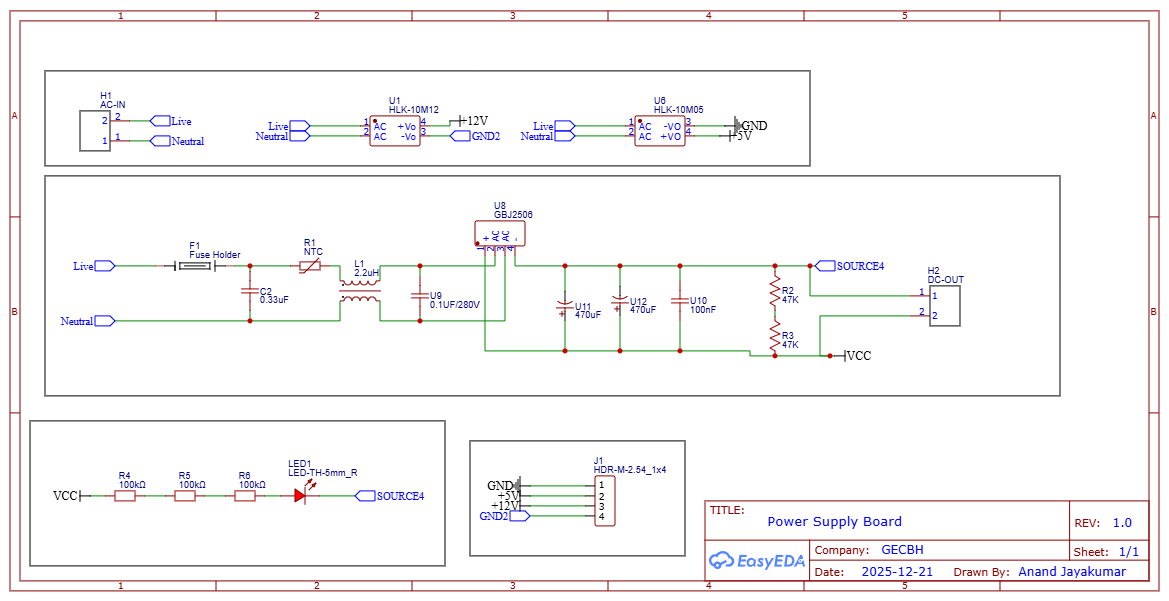
\includegraphics[width=1.1\linewidth]{./picture-files/PowerSupplyBoard/scheme.png}
\hfill
\caption{Schematics of the Power Supply Board}
\label{fig:PSscheme}
\end{figure}

\subsection{Non Discharging RCD Snubber Design}

A non-discharging RCD snubber is a passive snubber network used in power electronic converters to limit voltage spikes across the inverter MOSFETs. It typically consists of a resistor (R), capacitor (C), and diode (D) arranged so that the capacitor charges when a voltage spike occurs but does not discharge through the main switching device during the next switching cycle.

 The design of the non-discharge RCD snubber follows the methodology outlined by ROHM Semiconductor \cite{rohm_snubber_an} and the circuit figure is shown in figure \ref{fig:snubberdia}

 \begin{figure}[H]
\centering
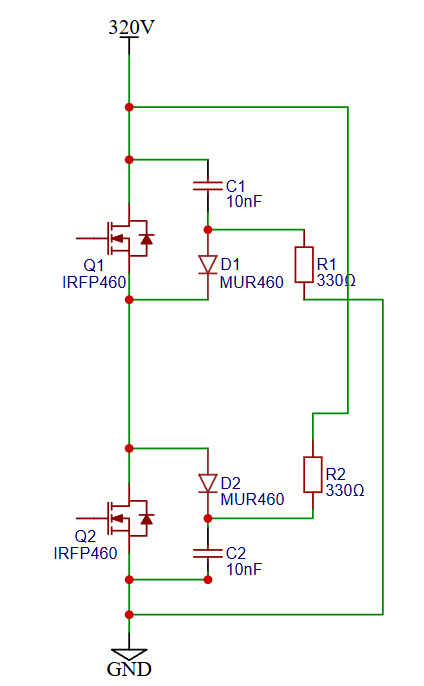
\includegraphics[width=0.4\linewidth]{./picture-files/snubberdia.png}
\caption[Snubber design]{Non discharging RCD snubber circuit for a half bridge.}
\label{fig:snubberdia}
\end{figure}


\subsubsection{Design requirement}
\begin{itemize}
    \item Operating frequency,f = 100 kHz
    \item DC Bus voltage, $V_\text{B}$ = 320 V
\end{itemize}

\subsubsection{Worst Case Design Calculations}
Assuming the following parameters:
\begin{itemize}
   \item Line inductance, $L_s = 10\mu\text{H}$
    \item Input current,  $I_o = 2.5\text{A}$
   \item Maximum allowable peak voltage,  $V_{pk} = 400\text{V}$ 
\end{itemize}


\subsubsection{Design Equations}
The peak voltage $V_{pk}$ is determined by the surge voltage $\Delta B$ added to the base voltage $V_B$:
\begin{equation}
    V_{pk} = \Delta B + V_B
\end{equation}

The surge voltage is calculated based on the leakage inductance $L_s$ and the snubber capacitance $C_{sn}$:
\begin{equation}
    \Delta B = I_o \sqrt{\frac{L_s}{C_{sn}}}
\end{equation}

Rearranging for the snubber capacitance $C_{SN}$:
\begin{equation}
    C_{SN} = \frac{I_o^2 \times L_s}{(V_{pk} - V_B)^2}
\end{equation}


\subsubsection{Snubber Capacitance}
Using the design formula, eq (3.3):
\[ C_{SN} = \frac{2.5^2 \times 10 \times 10^{-6}}{(400 - 320)^2} = 9.76 \times 10^{-9} \text{F} \approx 9.76\text{nF} \]
We select a standard value of \textbf{10nF}.

\subsubsection{Power Dissipation}
The power dissipated in the snubber is calculated at a frequency $f = 100\text{kHz}$:
\begin{equation}
     P = \frac{1}{2} C_{SN} (V_{pk} - V_B)^2 f 
\end{equation}
\[ P = \frac{1}{2} \times 10\text{nF} \times (400 - 320)^2 \times 100\text{kHz} = 3.2\text{W} \]

\subsubsection{Snubber Resistance}
To ensure the capacitor discharges within the switching period $t_{sw}$:
\begin{equation}
    R_{SN} < \frac{-t_{sw}}{C_s \times \ln \left[ \frac{V_{pk} - 0.9V_{pk}}{V_{pk}} \right]}
\end{equation}  
Substituting $t_{sw} = 10\mu\text{s}$ and $V_{pk} = 400\text{V} $ in eq (3.5):
\[ R_{SN} < 434.2 \, \Omega \]

\subsubsection{Confirmation of the design}
 The operating frequency is 100 kHz
\\ The time period, T is 10 $\mu s$
\\Time constant $\tau = {R_{SN} \times C_{SN}}$
 \\ For effective operation , $\tau$ must be between $\frac{T}{2}$ to $\frac{T}{10}$. That is between $1 \mu s$ to $5 \mu s$
\vspace{10pt}

From the designed value; $\tau = {10n F}\times {330\Omega}$ = 3.3 $\mu s$
\\This concludes that the design is valid adn ensures effective dampling of voltage spikes.

\vspace{10pt}

\subsubsection{Final Component Selection}
Based on the calculations, the selected components are:
\begin{center}

\begin{minipage}{0.4\textwidth}
    \textbf{Capacitor ($C_{SN}$):} 10nF \\
    \textbf{Resistor ($R_{SN}$):} 330$\Omega$, 5W \\
    \textbf{Diode:} MUR460
\end{minipage}

\end{center}

\vspace{10pt}

\subsection{High Voltage Transformer Design}
\label{sec-transformer}

\subsubsection{Design Requirements}
\begin{itemize}
    \item Input voltage: $V_\text{in,rms} = 320~\text{V}$
    \item Operating frequency: $f = 100~\text{kHz}$
    \item Output voltage: $V_\text{o,rms} = 3$--$4~\text{kV}$
    \item Output power: 200--300~W
    \item Target efficiency: $\eta \ge 90\%$
\end{itemize}

\subsubsection{Turns Ratio and Power Calculations}
\[
N = \frac{V_o}{V_\text{in}} = 12.5, \quad P_\text{in} =\frac{P_o}{\eta }\approx 333.33~\text{W}\quad I_\text{in} =\frac{P_o}{V_\text{in}} \approx 1.04~\text{A}, \quad I_o =\frac{P_o}{V_\text{O}} \approx 0.075~\text{A}
\]

\subsubsection{Core Selection and Turns}

\begin{equation}
\begin{aligned}
     A_p \ge \frac{V A}{2fJk_\text{w}B_\text{m}} 
\end{aligned}
\end{equation}

\[
     A_p \ge \frac{320 \times 1.04}{2\times 100k\times400\times0.4\times0.16} \ge 0.65~\text{cm}^4 
\]

\[   A_p (\text{selected}) = 13.45~\text{cm}^4 \textbf{(from the datasheet of the selected ETD-59 core)}\]

\[
    N_P=\frac{V_{in}}{4fB_\text{m}A_\text{e}}=\frac{320}{4\times 100k\times 0.16\times 368\times10^{-6}}= 14 turns
\]

\[
    N_s=\frac{V_{o}}{4fB_\text{m}A_\text{e}}=\frac{4000}{4\times 100k\times 0.16\times 368\times10^{-6}}= 170 turns
\]

\subsubsection{Conductor Selection and Skin Depth}
\begin{align*}
    \text{Skin depth: } \delta &= \frac{66.1}{\sqrt{f}} = \frac{66.1}{\sqrt{100\text{k}}} \approx 0.209 \text{ mm} \\
    \text{Maximum diameter} &= 2\delta = 2 \times 0.209 = 0.42 \text{ mm}
\end{align*}

\paragraph{For Primary:}
\begin{align*}
    A_{\text{cu}} &= \frac{I_{\text{in}}}{J} = \frac{1.04}{4} = 0.26 \text{ mm}^2 \\
    \text{Strand diameter } d &= \sqrt{\frac{4a}{\pi}} = 0.575 \text{ mm} > 0.42 \text{ mm}
\end{align*}

So we take a strand diameter of $0.27 \text{ mm}$. \par \raggedright

\begin{align*}
    \text{Area, } A &= \frac{\pi \times d^2}{4} = \frac{\pi \times 0.27^2}{4} = 0.0575 \text{ mm}^2 \\
    \text{No. of strands required} &= \frac{A_{\text{cu}}}{A} = \frac{0.26}{0.0575} = 4.5 \approx 5 \text{ strands}
\end{align*}

\paragraph{For Secondary:}
\begin{align*}
    A_{\text{cu}} &= \frac{I_0}{J} = \frac{0.075}{4} = 0.0188 \text{ mm}^2 \\
    \text{Strand diameter } d &= \sqrt{\frac{4a}{\pi}} = 0.15 \text{ mm}
\end{align*}

\subsection{Voltage and Current Sensing Module}

In order to monitor the operating conditions of the inverter system, a dedicated sensing module was designed to measure the DC link voltage and load current. The measured signals are conditioned and provided to the microcontroller analog inputs for monitoring and control purposes.

The designed sensing ranges are:

\begin{itemize}
\item \textbf{Voltage sensing range:} 0 -- 500 V DC
\item \textbf{Current sensing range:} 0 -- 3 A DC
\end{itemize}

Both sensing circuits employ galvanic isolation to protect the low voltage control circuitry from the high voltage power stage.

\subsubsection{Voltage Sensing Circuit}

The DC link voltage is sensed using a high value resistive voltage divider followed by an isolation amplifier.

\paragraph{Voltage Divider Network}

A resistor divider is used to scale the high voltage DC bus to a level suitable for the isolation amplifier input.

The divider consists of:\\
R1 = 560\,k$\Omega$, R2 = 560\,k$\Omega$, R3 = 470\,k$\Omega$, R4 = 470\,k$\Omega$, R5 = 470\,k$\Omega$, and R6 = 1\,k$\Omega$. \\

Total resistance:

\[
R_{total} = 560k + 560k + 470k + 470k + 470k + 1k
\]

\[
R_{total} = 2531k\Omega
\]

The divided voltage is taken across the lower resistor of the divider.

The voltage scaling ratio becomes:

\[
\frac{V_{out}}{V_{in}} = \frac{1k}{2531k}
\]

Thus the maximum sensed voltage becomes

\[
V_{out} = 500 \times \frac{1}{2531}
\]

\[
V_{out} \approx 0.198 V
\]

This reduced voltage is suitable for the isolation amplifier input.

\paragraph{Input RC Filter}

An RC filter is used at the divider output to remove switching noise from the inverter.

Components used:

\begin{multicols}{2}
\begin{itemize}
\item R = 68 $\Omega$
\item C = 0.01 $\mu$F
\end{itemize}
\end{multicols}

The cutoff frequency of the filter is

\[
f_c = \frac{1}{2\pi RC}
\]

\[
f_c = \frac{1}{2\pi (68)(0.01 \times 10^{-6})}
\]

\[
f_c \approx 234\,kHz
\]

This filter attenuates high frequency switching noise while allowing the DC voltage component to pass.

\paragraph{Isolated Power Supply}

To maintain electrical isolation between the high voltage sensing network and the control circuitry, an isolated DC-DC converter is used.

\textbf{B0505S isolated converter}

Specifications:

\begin{multicols}{2}
\begin{itemize}
\item Input voltage: 5 V
\item Output voltage: 5 V isolated
\item Isolation voltage: 1 kV
\item Output power: 1 W
\end{itemize}
\end{multicols}

This ensures that the sensing amplifier input side remains electrically isolated from the microcontroller side.

\paragraph{Isolation Amplifier}

The sensed voltage is measured using the \textbf{HCPL-7800 isolation amplifier}.

Important specifications of HCPL-7800:

\begin{multicols}{2}
\begin{itemize}
\item Isolation voltage: 3.75 kV
\item Bandwidth: 100 kHz
\item Differential input range: $\pm 200$ mV
\item Gain accuracy: $\pm 1\%$
\item Low non-linearity
\end{itemize}
\end{multicols}

The amplifier converts the differential input voltage into an isolated output voltage.

The simplified transfer relation is:

\[
V_{out} = G \times (V_{IN+} - V_{IN-})
\]

where

\begin{itemize}
\item $G$ is the internal gain of the isolation amplifier
\item $V_{IN+}$ and $V_{IN-}$ are the differential input voltages
\end{itemize}

\paragraph{Signal Conditioning using Operational Amplifier}

The output of the isolation amplifier contains a DC offset that must be removed before it is fed to the microcontroller ADC.

An operational amplifier (MCP6002) configured in differential mode is used to remove this offset and scale the signal.

Resistors used:

\begin{multicols}{2}
\begin{itemize}
\item R8 = 10 k$\Omega$
\item R9 = 20 k$\Omega$
\item R10 = 10 k$\Omega$
\item R11 = 20 k$\Omega$
\end{itemize}
\end{multicols}

The gain of the differential amplifier is

\[
A_v = \frac{R9}{R8}
\]

\[
A_v = \frac{20k}{10k}
\]

\[
A_v = 2
\]

Thus the final output voltage becomes

\[
V_{MCU} = 2(V_{out+} - V_{out-})
\]

The conditioned signal is then fed to the analog input of the microcontroller.

\subsubsection{Current Sensing Circuit}

The current sensing circuit measures load current using the shunt resistor method.

\paragraph{Current Shunt}

A precision shunt resistor is placed in series with the load.

Shunt value:

\[
R_{shunt} = 40m\Omega
\]

Maximum measurable current:

\[
I_{max} = 3A
\]

The maximum shunt voltage becomes

\[
V_{shunt} = I \times R
\]

\[
V_{shunt} = 3 \times 0.04
\]

\[
V_{shunt} = 0.12V
\]

Thus the shunt produces a maximum voltage of \textbf{120 mV}.

\paragraph{Isolation Amplifier}

The differential shunt voltage is measured using the same \textbf{HCPL-7800 isolation amplifier}. This allows safe measurement of current flowing in the high voltage DC link.

The amplifier provides galvanic isolation between the power stage and control circuitry.

\paragraph{Signal Conditioning}

The amplifier output is processed using the second operational amplifier contained in the same \textbf{MCP6002 dual op-amp package}.

Resistors used:

\begin{multicols}{2}
\begin{itemize}
\item R15 = 10 k$\Omega$
\item R16 = 10 k$\Omega$
\item R14 = 33 k$\Omega$
\item R17 = 33 k$\Omega$
\end{itemize}
\end{multicols}

The gain of this stage is

\[
A_v = \frac{R14}{R15} = \frac{33k}{10k} = 3.3
\]



Thus the conditioned current signal provided to the microcontroller becomes

\[
V_{MCU} = 3.3 \times V_{shunt}
\]

For the maximum current of 3 A:

\[
V_{MCU} = 3.3 \times 0.12
\]

\[
V_{MCU} = 0.396V
\]

This voltage lies safely within the input range of the microcontroller ADC.

\subsubsection{Operational Amplifier}

Both signal conditioning stages use the \textbf{MCP6002 operational amplifier}. This device contains two operational amplifiers within the same package.

Important features:

\begin{multicols}{2}
\begin{itemize}
\item Dual operational amplifier
\item Rail-to-rail input and output
\item Supply voltage range: 1.8 V – 6 V
\item Low power consumption
\item Suitable for microcontroller ADC interfacing
\end{itemize}
\end{multicols}

Using a dual op-amp reduces component count and PCB area while allowing both voltage and current signals to be conditioned using a single IC.

\begin{figure}[h!]
\centering
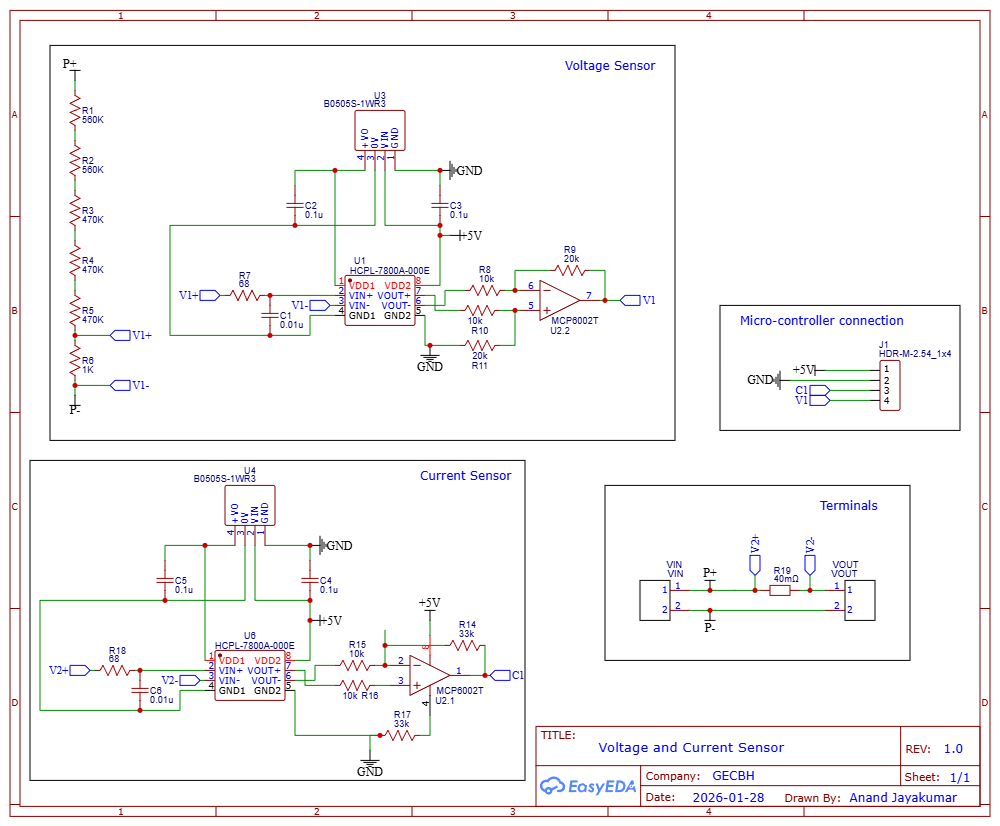
\includegraphics[width=1.1\linewidth]{./picture-files/Sensors/Schematic_v-and-current-sensor.png}
\caption[Voltage and Current Sensor Schematics]{Voltage and Current Sensor Schematics}
\label{fig-cw}
\end{figure}


\subsection{Cockcroft--Walton Voltage Multiplier Design}
To achieve the 30 kV DC target output from a 4 kV AC input, a multi-stage Cockcroft--Walton multiplier is employed. This design scales the voltage according to the number of stages $n$
\\[.75cm]
Input peak voltage, $V_{\text{peak}}$ = 4 kV (output from the transformer)
\\Approximate output voltage required, $V_{\text{out}}$ = 30 kV
\begin{multicols}{2}
\begin{itemize}
\item Selected capacitors: 1~nF, 15~kV
\item Selected diodes: 2CL2FL, 15~kV, 5~mA
\end{itemize}
\end{multicols}

The output voltage is calculated as:
\begin{equation}
    V_{\text{out}} \approx 2n V_{\text{peak}}
\end{equation}
\[
    n = \frac{30\,\text{kV}}{2 \times 4\,\text{kV}} = 3.75 \approx 4 \text{ stages}
\]

\begin{figure}[h!]
\centering
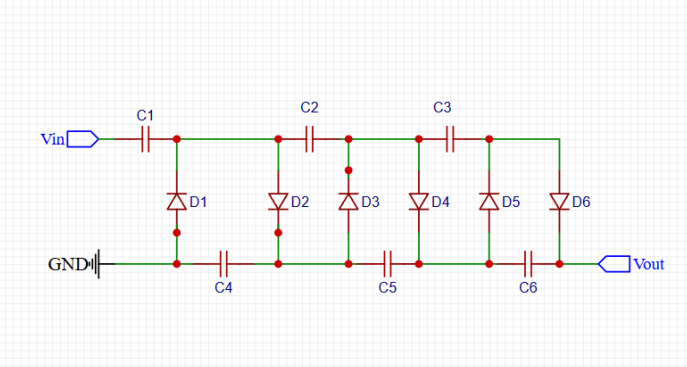
\includegraphics[width=0.9\linewidth]{./picture-files/cock.png}
\caption[3 Stage-Cockcroft Walton Generator]{3 Stage-Cockcroft Walton Generator}
\label{fig-cw}
\end{figure}

\pagebreak

\section{Summary}
A complete high-voltage cold plasma generation system was designed consisting of the following key subsystems:

\begin{enumerate}
    \item UCC21330 isolated gate driver circuit for H-bridge switching  
    \item Power supply board providing 5 V, 12 V, and 320 V DC rails  
    \item Non-discharging RCD snubber for protection against voltage spikes  
    \item High-frequency high-voltage transformer (3--4 kV, 100 kHz)  
    \item Cockcroft--Walton voltage multiplier generating 30 kV DC  
    \item Voltage and current sensing module with isolation and signal conditioning  
\end{enumerate}